\section{Introduction papier demouillage}
Le solvant, autrefois considéré comme secondaire, apparait de plus en plus important dans le rôle et la stabilité aussi bien de petits composés chimiques\cite{khamar_investigating_2014} que de gros assemblages biologiques \cite{prabhu_proteinsolvent_2006, kuhrova_are_2014, schwabe_role_1997}. Les méthodes de modélisation moléculaire représentant le solvant de façon explicite, consacrent la majeure partie de leur temps aux calculs des interactions solvant-solvant. Ces méthodes sont donc limitées aux systèmes de petites tailles. Afin d'étudier des plus gros systèmes, différents modèles implicites\cite{roux_implicit_1999} ont été proposés. Certains d'entre eux permettent de prédire les propriétés structurelles et thermodynamiques des fluides moléculaires avec une précision équivalente aux méthodes explicites telles que les méthodes de dynamiques moléculaires (DM) ou de monte carlo (MC) avec un coup numérique inférieur de plusieurs ordres de grandeurs.



Parmis ces méthodes implicites, une des méthodes les plus utilisées est the integral equation theory in the molecular picture\cite{blum_invariant_1972,blum_invariant_1972-1}. Cette méthode est cependant limitée et ne peut pas être utilisée pour des solutes complexes en 3 dimensions. Une approximation de cette méthode a également été développée, the reference interaction site model (RISM)\cite{chandler_optimized_1972,hirata_application_1982} puis dérivée dans une version adaptée aux solutés complexes en 3 dimensions 3DRISM\cite{beglov_integral_1997,hirata_molecular_2003}. Ces méthodes restent cependant approximatives car elles considèrent les molécules comme un ensemble de sites indépendants. Afin de dépasser ces limites, Jeanmairet et Al. ont proposé une nouvelle théorie, moléculaire et adaptée à n'importe quel soluté de n'importe quelle forme: the Molecular Density Functional Theory (MDFT) \cite{ramirez_density_2002, ramirez_direct_2005, ramirez_density_2005, gendre_classical_2009, zhao_molecular_2011, borgis_molecular_2012, levesque_scalar_2012, levesque_solvation_2012, jeanmairet_molecular_2013-1}. La théorie de la fonctionnelle de la densité moléculaire (MDFT), basée on the homogeneous reference fluid approximation (HRF), consiste à minimiser une énergie libre de solvatation qui est une fonctionnelle de la densité locale de solvant (ici d'eau SPC/E)\cite{berendsen_missing_1987}. Cette théorie soeur de la Kohn-Sham DFT \cite{kohn_self-consistent_1965} pour les électrons s'exprime ici pour une densité (classique, ie non quantique) de molécules d'eau. On note cette densité  $\rho(\vec{r})$, qui a la dimension d'un nombre de molécules de solvant par unité de volume. D'excellentes revues et cours ont été écris par Evans \cite{evans_nature_1979,evans_density_2009,henderson_fundamentals_1992}.

La Gibbs free energy of solvation functional s'exprime 
\begin{equation} \label{eq:fonctionale_globale}
F[\rho(\vec{r})]=F_{\mathrm{id}}+F_{\mathrm{ext}}[\rho(\vec{r})]  +  F_{\mathrm{exc}}[\rho(\vec{r})]
\end{equation}
avec
\begin{eqnarray}
\beta \mathcal{F}_\mathrm{id} &=& \int \rho(\vec{r}) \ln\left(\frac{\rho(\vec{r})}{\rho_0}\right)-\rho(\vec{r})+\rho_0  \mathrm{d}\vec{r} \\
\mathcal{F}_\mathrm{ext} &=& \int  f_\mathrm{ext}(\vec{r}) \rho(\vec{r}) \mathrm{d}\vec{r} \\
\beta \mathcal{F}_\mathrm{exc} &=& -\frac{1}{2} \iint \Delta\rho c(\vec{r},\vec{r}^\prime) \Delta\rho \mathrm{d}\vec{r} \mathrm{d}\vec{r}^\prime + \mathcal{F}_\mathrm{B}
\end{eqnarray}
avec $\rho_0$ la densité bulk de solvent (soit 0.0333 molécules/$\text{\AA}^3$ ou 1kg/L pour l'eau), $\Delta\rho(\vec{r})=\rho(\vec{r})-\rho_0$, $c(\vec{r}, \vec{r}')$ la fonction de correlation direct de l'eau et $\mathcal{F}_\mathrm{B}$ la fonctionnelle de bridge contenant tous les termes d'ordres supérieurs à 2 dans le développement autour de $\rho_0$ de la fonctionnelle d'excès. Une description des dernières avancées du calcul de la partie HRF est disponible dans le papier de Jeanmairet et Al\cite{jeanmairet_molecular_2016}.





\section{blabla}
The molecular density functional theory permet de calculer l'énergie libre de solvatation ainsi que l'organisation du solvent autour d'un composé de n'importe quelle forme lorsqu'on le plonge dans notre modèle d'eau. Habituellement, la fonctionnelle est une fonction de la densité en chaque point $\vec{r}$ de l'espace et pour chaque orientation $\omega$ du solvent. 






\section{PBC}
\begin{tikzpicture}

% water molecule in the initial simulation box
\path (0.45,3.3) node {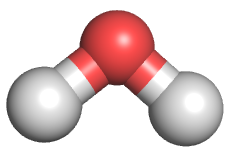
\includegraphics[width=0.75cm]{images/wat}}
      (1.6,4.4)  node {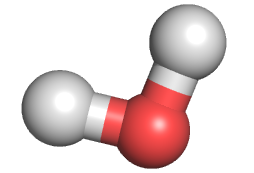
\includegraphics[width=0.75cm]{images/wat3}}
      (0.5,4.45) node {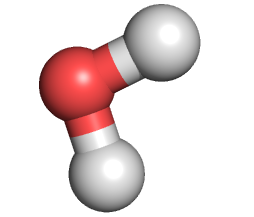
\includegraphics[width=0.75cm]{images/wat2}}
      (1.1,3.7)  node {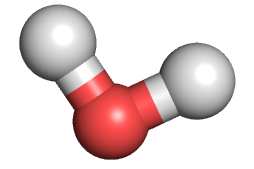
\includegraphics[width=0.75cm]{images/wat4}};

% edge of the initial simulation box
\path[draw,ultra thick] (0,3) rectangle (2,5);

% periodic boundaries
\foreach \x in {5,7,9} {
    \foreach \y in {1,3,5} {
        % water molecules in images
        \node at (\x+0.45,\y+0.3) {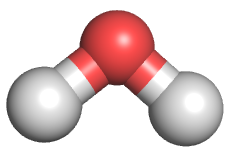
\includegraphics[width=0.75cm]{images/wat}};
        \node at (\x+1.6 ,\y+1.4) {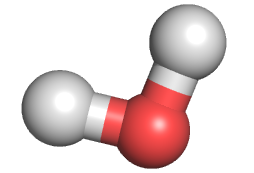
\includegraphics[width=0.75cm]{images/wat3}};
        \node at (\x+0.5 ,\y+1.45) {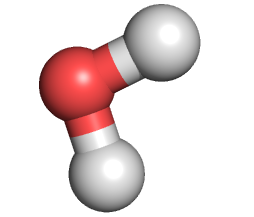
\includegraphics[width=0.75cm]{images/wat2}};
        \node at (\x+1.1 ,\y+0.7) {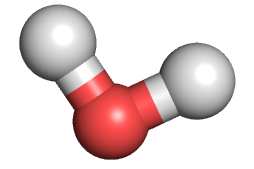
\includegraphics[width=0.75cm]{images/wat4}};
        
        % edge of each box
        \path[draw,thick] (\x,\y) rectangle (\x+2,\y+2);
    }
}

% central box thicker than other
\path[draw,ultra thick] (7,3) rectangle (9,5);

% an arrow
\path[draw,ultra thick,->] (2.5,4) -- (4.5,4);

% dashed lines 
\foreach \x in {5,7,9,11} {
    % vertical
    \path[draw,dashed,thick] (\x,0) -- (\x,1) (\x,7) -- (\x,8);
    % horizontal
    \path[draw,dashed,thick] (4,\x-4) -- (5,\x-4) (11,\x-4) -- (12,\x-4);
}

\end{tikzpicture}

